\chapter{Introduction} \label{chap:intro}
``The most profound technologies are those that disappear.'', Mark Weiser, Chief Technologist at Xerox PARC, famously wrote in his \textit{The Computer for the 21st Century} (\citeyear{weiser1991computer}) \cite{weiser1991computer}. Indeed, the vision of ubiquitous computing, or \mbox{\textbf{ubicomp}}, which he largely coined, is one where computers are invisible servants merged with the environment. They inform the user without requiring their attention, and controlling them is intuitive to the point where they feel like an extension of the user's unconsciousness rather than a tool \cite{weiser1997coming}.

One of the first examples of ubicomp was the now-famous ``Live Wire'' or ``Dangling String'', shown in Figure \ref{fig:live_wire}. It is an ordinary piece or rope attached to a motor which is linked to a computer network. Whenever some data is transmitted over the network, the motor is activated and the wire starts to twitch. The more data is being transmitted, the more intensely the wire twitches. It is a perfect example of ``\mbox{\textbf{Calm Technology}}'', a form of technology that resides mainly in the periphery. Indeed, the wire will never interrupt the user's activities or force their attention, but users may notice the twitching from their peripheral vision and decide to look at their own leisure. Calm technology is a core concept in ubicomp, because it is always available but never interrupts the user, it offers a service without demanding attention \cite{weiser1996designing}.

\begin{figure}
    \centering
    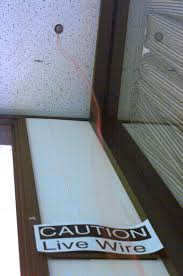
\includegraphics[width=0.3\linewidth]{introduction/live_wire.jpg}
    \caption{A Live Wire hanging from the ceiling \cite{weiser1996designing}}.
    \label{fig:live_wire}
\end{figure}

In the years following the conception of ubicomp, research and industry progressed far beyond the point of dangling strings. At the turn of the milennium we saw the emersion of digital clocks that not just display time but also the weather forecast, the room temperature, and other information. Of course, clocks were already a form of ubicomp in and of themselves, continuously telling the time without forcing the user's attention, and weather forecasts were available in a variety of ways. However, having all this information neatly summarized, available at a glance when we get up in the morning, was revolutionary in its own right.

\todo{One more paragraph on ubicomp to explain the current state of the technology, then below talk about the history of AR.}

For decades, a big obstacle, if not \textit{the} biggest one, in the further development of ubicomp, has been hardware capabilities; low power consumption, solid wireless communication and excellent (touch) displays are but some of the requirements for enabling the seamless human-computer interaction that Weiser and others envisioned \cite{weiser1993some}. In recent years, however, these hurdles are being rapidly overcome. The widespread adoption of smartphones, which boast all three of the aforementioned requirements, is perhaps the most striking evidence thereof.

With hardware limitations diminishing, other ubicomp challenges are becoming more prominent. Some current open research questions concern \textbf{intelligibility}, or how to make computer systems easy to understand, and visibility, or how to make users aware of the presence of these systems \cite{vermeulen2009bet,vermeulen2013intelligibility}. The fact that computers being too small to see is now a concern, goes to show just how much progress has been made.

The solution to the usability problems of ubicomp might, somewhat counterintuitively, be to hide the computer entirely. The idea behind virtual reality (VR) and augmented reality (\textbf{AR}) is for the computer to become completely invisible by taking control of the user's sensory input, which at the same time would allow it to communicate using any combination of visual, auditory and other signals \cite{rheingold1991virtual}. As such, the computer would be able to convey information intuitively and with any degree of intrusiveness, making the approach excellent for implementing the ubicomp ideals \cite{weiser1993some}.

Another challenge in ubicomp concerns the fact that, while actions in virtual environments are often reversible, the real world is much less forgiving. For this reason, it's essential to inform users of what actions will achieve which effect in a process called \textbf{feedforward} \cite{djajadiningrat2002but}. While the notion of feedforward is both powerful and important, much research on the topic remains to be done \cite{vermeulen2013crossing}.

In this thesis, we investigate the potential of AR for giving feedforward on ubicomp systems, with the goal of improving their intelligibility. More specifically, we look for intuitive cues that can inform the user on the result of each possible action they can take in a given environment. Feedforward via senses other than vision, such as auditory or tactile input, are not considered.

\todo{The description of chapters below must be adjusted.}

Chapter \ref{chap:explor} commences this thesis with a study of related work. We look at interaction techniques concerning AR, feedforward and ubicomp that are suggested by other research teams and analyze the results of past experiments on these topics. Using that information, we look for an interesting problem on which we can perform an in-depth study for the remainder of this thesis.

The problem that we decide on is the spatial mapping problem of light switches, or the question of which lights are connected to which switches in a given room (and vice versa). We chose this problem because it is both relevant and recognizable, since many people need to solve such problems on a regular basis, and because it allows us to easily come up with scenarios of arbitrary complexity.

Our next step is to gather initial data on a wide variety of solutions so as to better focus the remainder of our study. To this end, we distribute an online survey containing seven different visualizations, and for each of them, we measure the performance and perception of the respondents. The setup, execution, results and conclusions of this preliminary study are discussed in chapter \ref{chap:explor}.

%In 1988, when I started PARC’s work on ubiquitous computing, virtual reality (VR) came the closest to
%enacting the principles we believed important. In its ultimate envisionment, VR causes the computer to
%become effectively invisible by taking over the human sensory and affector systems [Rheingold 91]. VR
%is extremely useful in scientific visualization and entertainment, and will be very significant for those
%niches. But as a tool for productively changing everyone’s relationship to computation, it has two crucial
%flaws: first, at the present time (1992), and probably for decades, it cannot produce a simulation of
%significant verisimilitude at reasonable cost (today, at any cost). This means that users will not be fooled
%and the computer will not be out of the way. Second, and most importantly, it has the goal of fooling the
%user -- of leaving the everyday physical world behind. This is at odds with the goal of better integrating
%the computer into human activities, since humans are of and in the everyday world. \cite{weiser1993some}

%Human-computer interaction has come a long way since the first computers were created around 75 years ago. 
%We've come a long way since the invention of computers
%Interfaces have changed a lot, and now, like the devices they belong to, they're becoming ubiquitous.
%New interface require new techniques
%Many techniques have been developed over the years: affordances and signifiers, (continuous) feedback and feedforward
%Actions in the real world are not always as reversible as they are in the virtual world.

%\section{Feedforward} \label{section_background}
%Feedforward is a relatively new concept that has been the subject of much confusion, and thus it is worth clarifying. Feedforward was first defined by \citeauthor{djajadiningrat2002but} in \citeyear{djajadiningrat2002but} as 
%
%
%Feedforward is:
%	communication of the purpose of an action. \cite{djajadiningrat2002but}
%
%	informs the user about what the result of his action will be. Inviting the appropriate action is a prerequisite for feedforward but it is not sufficient. The product also needs to communicate what the user can expect. \cite{djajadiningrat2002but}
%
%	a HCI design technique that aims at making explicit the action that is required to perform an interaction and its effect. \cite{chueke2016perceptible}
%	
%	intelligibility information that is provided before an event takes place. \cite{vermeulen2013intelligibility}
%	
%	communicating what will be the result of an action


%Feedforward hasn't always been clearly defined. People don't know it exists, confuse it with other concepts (like affordances) or use different names for it (signifiers). Let's now define what feedforward is, according to different definitions.
%
%Perceptible affordances and feedforward for gestural interfaces: Assessing effectiveness of gesture acquisition with unfamiliar interactions \cite{chueke2016perceptible}
%
%Intelligibility Required: How to Make Us Look Smart Again \cite{vermeulen2013intelligibility}
%
%Crossing the bridge over Norman's Gulf of Execution: revealing feedforward's true identity \cite{vermeulen2013crossing}
%
%When it is not possible for designers of electronic products to establish direct couplings between action and function information is needed. Information that can guide the user’s actions towards the intended function. This is the area of feedback and feedforward. \cite{wensveen2004interaction}
%
%With feedforward we mean communication of the purpose of an action. \cite{djajadiningrat2002but}
%
%For a control to say something about the function that it triggers, we need to move away from designs in which all controls look the same. \cite{djajadiningrat2004tangible} 
%
%As pointed out by Norman \cite{norman2013design}, controls of electronic products often look highly similar and require the same actions. If all controls look the same and feel the same, the only way left to make a product communicate its functions is through icons and text labels, requiring reading and interpretation. \cite{djajadiningrat2004tangible}
%
%Signifiers are the most important addition to the chapter, a concept first introduced in my book Living with Complexity. The first edition had a focus upon affordances, but although affordances make sense for interaction with physical objects, they are confusing when dealing with virtual ones. As a result, affordances have created much confusion in the world of design. Affordances define what actions are possible. Signifiers specify how people discover those possibilities: signifiers are signs, perceptible signals of what can be done. Signifiers are of far more importance to designers than are affordances. Hence, the extended treatment. \cite{norman2013design}
%
%Preview important in the real world because it is often not possible to undo an action. \cite{rekimoto2003presense}
